\documentclass{article}
\usepackage[utf8]{inputenc}
\usepackage[parfill]{parskip}
\usepackage{hyperref}
\usepackage{graphicx}
\graphicspath{ {images/} }

\usepackage{subcaption}
\usepackage{amsfonts}

\title{CS394R\@: Programming Assignment 4}
\author{Ashish Bora}
\date{November 2016}

\usepackage{hyperref}
\hypersetup{
    colorlinks=true,
    linkcolor=blue,
    filecolor=magenta,
    urlcolor=cyan,
}

\begin{document}

\maketitle

\section{Abstract}

In this programming assignment, we introduce a modification to the semi-gradient $TD(0)$ algorithm for approximating the state value function. We compare the new method to Monte Carlo and $TD(0)$ methods empirically on a random walk task. Code used for this assignment can be found at \url{https://github.com/AshishBora/reinforcement-learning}.

\section{Introduction}

Real world reinforcement learning problems often have very large state spaces. In order to efficiently learn the optimal actions in such scenarios, function approximation is regularly deployed. A typical way of applying this is to assume a representation for the states and/or actions and use a parametrized function that maps these representations to either state values or state-action values. In this work, we will consider only state value functions. The task is thus to find parameter values such that the resulting function is a ``good'' approximation of the true value function of a given policy $\pi$.

Since the function approximation will typically not be able to model all the state values accurately, it will invariably make some errors on some states. Thus, to be able to pick good parameter values, we also need to specify which kind of errors we prefer. This is typically done via a loss function which we then seek to minimize.

Let us denote the true value function by $v_{\pi}(s)$ and the approximation to it by $\hat{v}(s, \theta)$, where $\theta$ are the parameters of the approximation function. Let $d(s)$ denote the fraction of time spent in state $s$ under the policy $\pi$. It is common to use the following loss function:
$$MSVE(\theta) = \sum_{s \in \mathcal{S}} d(s) {\left[v_{\pi}(s) - \hat{v}(s, \theta) \right]}^2$$

This objective can also be seen as an expectation of the squared error over time as the agent moves around the state space.\ i.e.

\begin{equation}\label{eqn1}
MSVE(\theta) =  \lim_{T \rightarrow \infty} \mathbb{E} \left[ \frac{1}{T} \sum_{t=1}^{T} {\left( v_{\pi}(S_t) - \hat{v}(S_t, \theta) \right)}^2 \right]
\end{equation}

There are several ways of minimizing this objective. Monte Carlo and semi-gradient $TD(0)$ methods have been proposed for the same. In this work, we will look at a new method which is a slight modification of the semi-gradient $TD(0)$ method.

In the next section, we introduce Monte Carlo and semi-gradient $TD(0)$ algorithms. Using this, we try to develop intuition about what these algorithms are trying to do, which will then lead to the new algorithm. Finally, we empirically compare these algorithms in the random walk environment.

\section{Monte Carlo algorithm}

This algorithm poses the problem of finding good values for parameter values $\theta$ as a supervised learning task and treats the returns ($G_t$) obtained from each episode to be examples of the form $(S_t, G_t)$ for that purpose.

The gradient of $MSVE$ with respect to $\theta$ is
$$\nabla MSVE(\theta) = \sum_{s \in \mathcal{S}} 2 d(s) \left[ v_{\pi}(s) - \hat{v}(s, \theta) \right] \nabla \hat{v}(s, \theta) $$

We can replace the sum over states by random walk given by the episode since it has the same distribution in expectation. This gives
$$\nabla MSVE(\theta) = 2 \mathbb{E} \left[ \left( v_{\pi}(S_t) - \hat{v}(S_t, \theta) \right) \nabla \hat{v}(S_t, \theta) \right] $$

Further, we can replace $v_{\pi}(S_t)$ by $G_t$ since it is an unbiased estimator of $v_{\pi}(S_t)$. This yields the Monte Carlo algorithm shown in Fig.~\ref{fig:mc_alg}.
\begin{figure}[ht!]
    \centering
    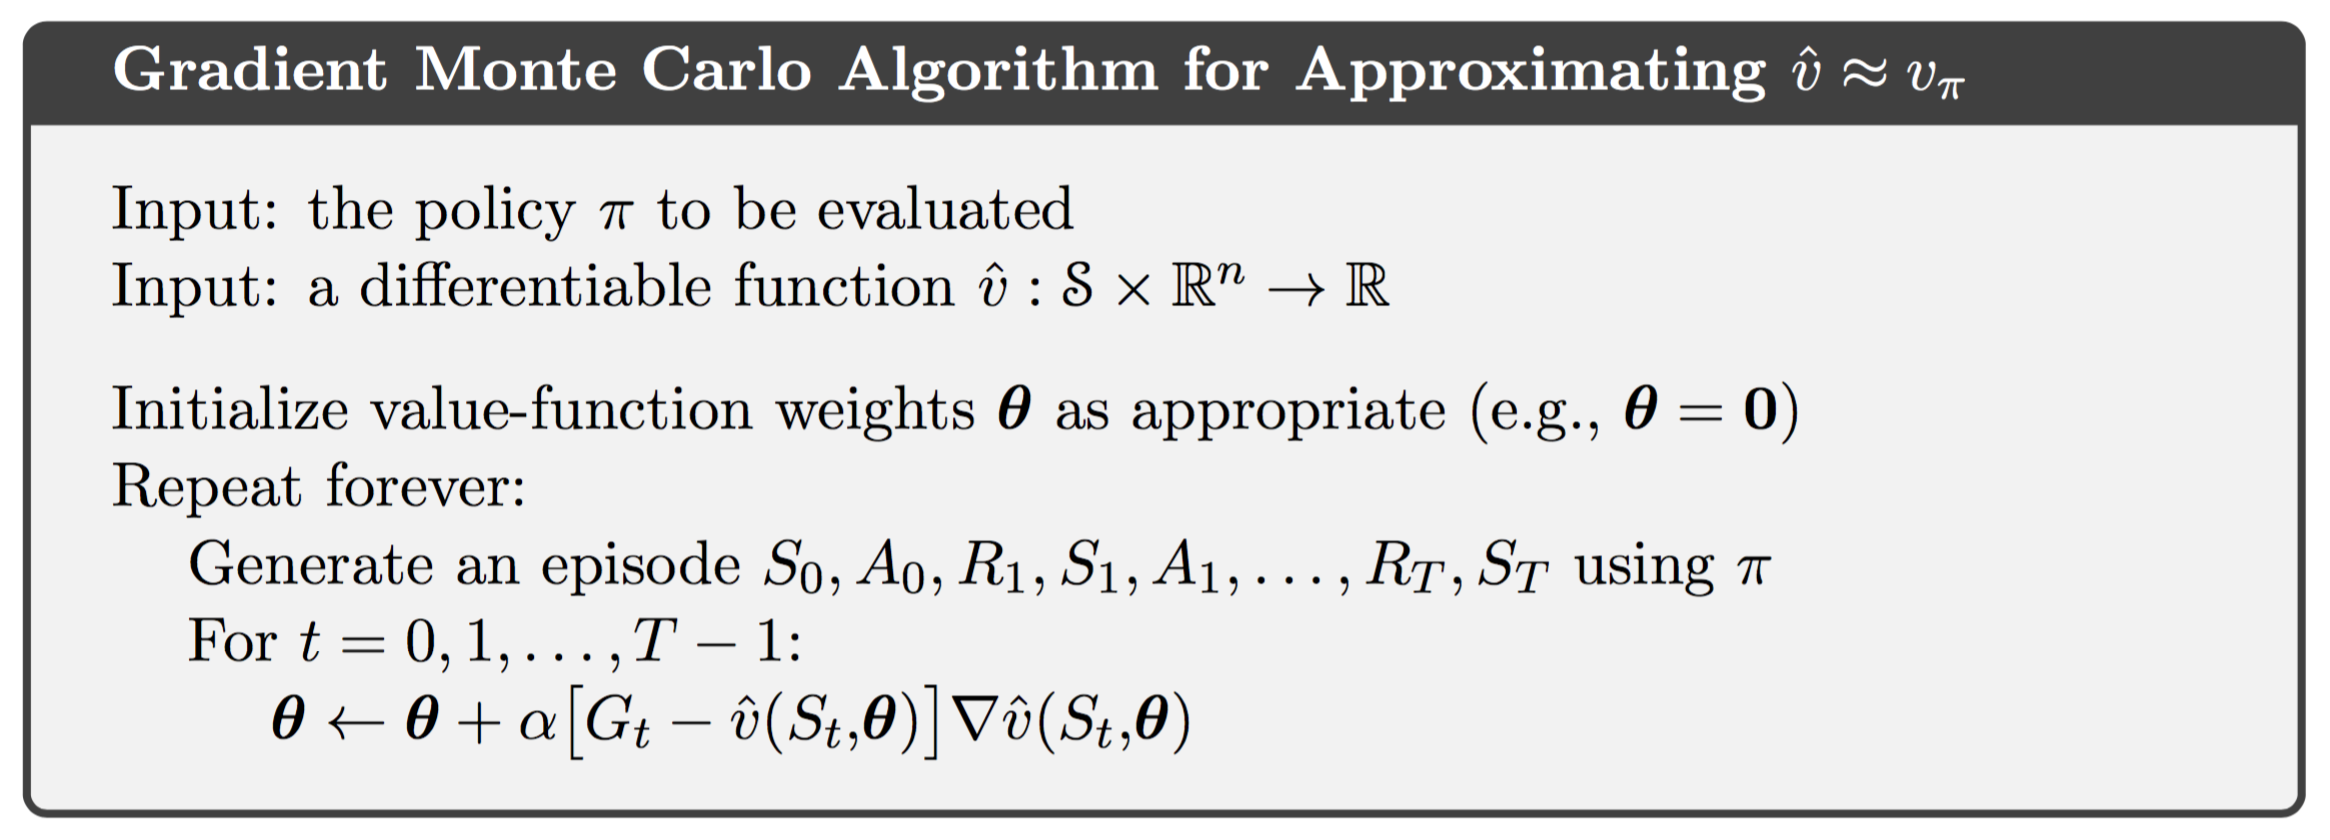
\includegraphics[width=\textwidth]{mc_alg}
    \caption{From~\cite{RLbook}}\label{fig:mc_alg}
\end{figure}
Since the expectation of the gradient is same as the true gradient, we note that this is an instance of stochastic gradient descent to optimize $\theta$.

\section{semi-gradient $TD(0)$ algorithm}

Instead of waiting for the episode to finish, this algorithm tries to make updates quickly. To do this, it uses bootstrapping. Thus, instead of replacing $v_{\pi}(S_t)$ values by $G_t$, they are replaced by the bootstrapped estimate given by the next step, i.e. $R + \gamma \hat{v}(S_{t+1}, \theta)$. This leads to the algorithm shown in Fig.~\ref{fig:semi_alg}.
\begin{figure}
    \centering
    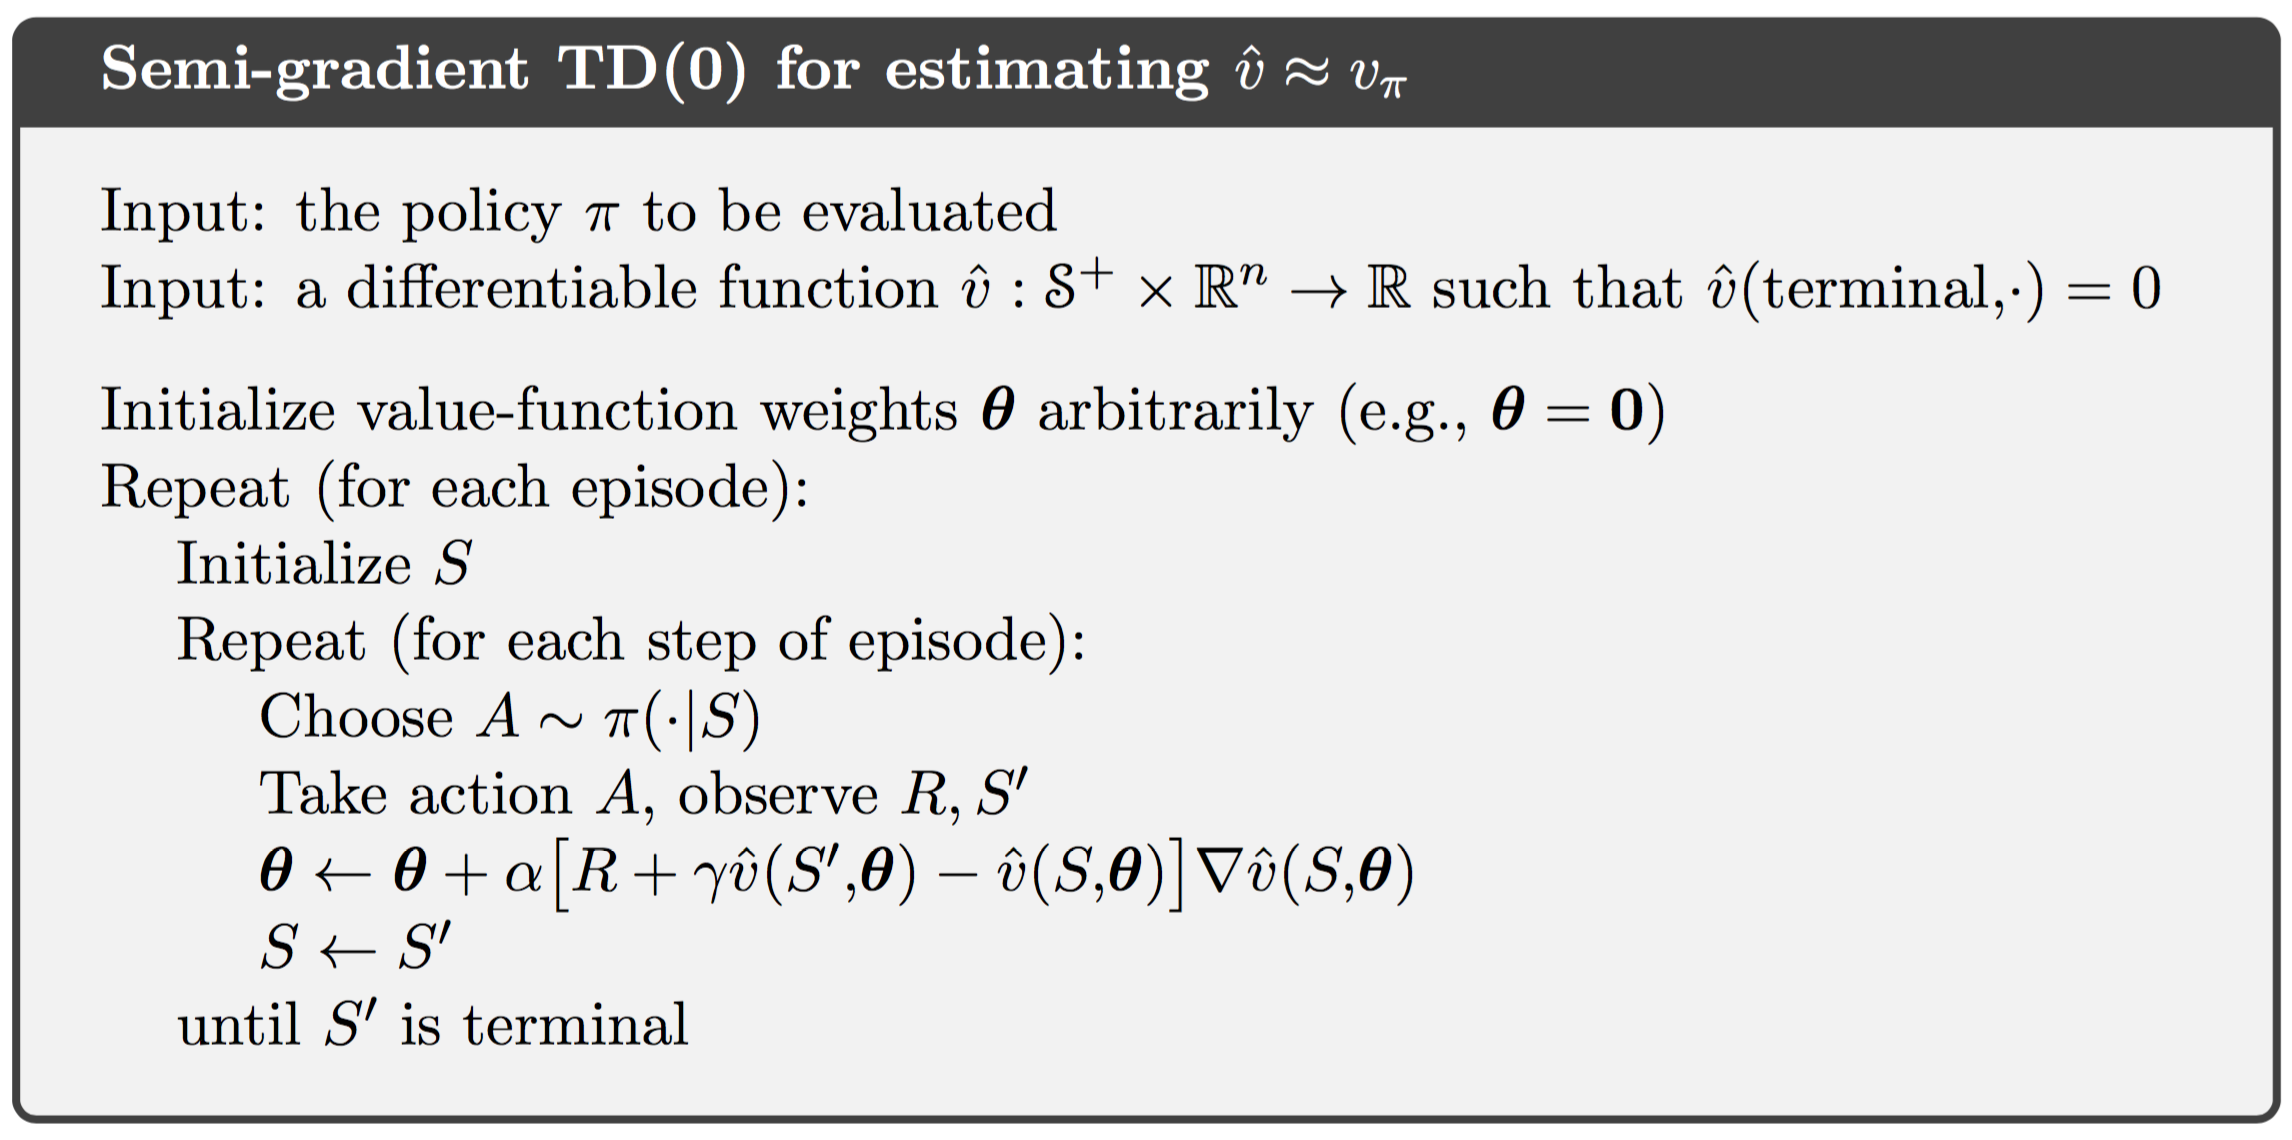
\includegraphics[width=\textwidth]{semi_alg}
    \caption{From~\cite{RLbook}}\label{fig:semi_alg}
\end{figure}

This algorithm is called semi-gradient because it not the actual gradient of $MSVE$\@. Usage of bootstrapped values means that we account for only a portion of the gradient.

\section{demi-gradient $TD(0)$ algorithm}

Semi-gradient $TD(0)$ algorithm can be understood as trying to change the value of $S_t$ such that it is closer to the bootstrapped estimate. Unfortunately this has to be done through function approximation and thus may end up changing values for other states as well, which may in fact increase the gap between the bootstrapped estimate and the approximated value.

We observe that this problem occurs because while constructing the algorithm, we simply replaced $G_t$ by the bootstrapped estimate $R + \gamma \hat{v}(S_{t+1}, \theta)$, even though its expectation was not equal to the true return. Thus this algorithm is not trying to minimize the $MSVE$, but something else.

To better understand what is being minimized, we construct a new $MSVE$ that is well motivated and leads to a gradient based update of a form ``similar'' to the semi-gradient method. From equation (\ref{eqn1}), we have
$$MSVE(\theta) =  \lim_{T \rightarrow \infty} \mathbb{E} \left[ \frac{1}{T} \sum_{t=1}^{T} {\left( v_{\pi}(S_t) - \hat{v}(S_t, \theta) \right)}^2 \right]$$

An alternative formulation is thus to use bootstrapped estimates:
$$MSVE_2(\theta) = \lim_{T \rightarrow \infty} \mathbb{E} \left[ \frac{1}{T} \sum_{t=1}^{T} {\left( R_{t+1} + \gamma \hat{v}(S_{t+1}, \theta) - \hat{v}(S_t, \theta) \right)}^2 \right]$$

Note that this formulation is well motivated since the recursive equations
$$\hat{v}(S_t, \theta) = \mathbb{E}_{\pi} \left[ R_{t+1} + \gamma \hat{v}(S_{t+1}, \theta) \right]$$
have a unique fixed point which is the same as the actual value function $v_{\pi}$.

The gradient of this loss with respect to $\theta$ is thus
$$2 \lim_{T \rightarrow \infty} \mathbb{E} \left[ \frac{1}{T} \sum_{t=1}^{T} \left( R_{t+1} + \gamma \hat{v}(S_{t+1}, \theta) - \hat{v}(S_t, \theta) \right) (\gamma \nabla \hat{v}(S_{t+1}, \theta) - \nabla \hat{v}(S_t, \theta))\right].$$

So, we can see that the semi-gradient update rule is derived from this \emph{if we ignore} the $\gamma \nabla \hat{v}(S_{t+1}, \theta)$ term. Thus semi-gradient uses an update that is partial at two levels, first it changes the objective a little bit and then it takes only part of the gradient of the new objective. The first step is justified due to the value iteration fixed point theorem, but the second step seems arbitrary.

Thus, the modification proposed in this work is to use the full gradient of the modified objective. This is still a partial gradient time difference method, since we are using bootstrapped values, and thus is accordingly named demi-gradient $TD(0)$.

An intuitive way of thinking about this is the following:
semi-gradient $TD(0)$ is trying to update $\hat{v}(S_{t}, \theta)$ such that it is closer to the bootstrapped estimate. Demi-gradient $TD(0)$ on the other hand allows itself the freedom to change both $\hat{v}(S_{t}, \theta)$ and $\hat{v}(S_{t+1}, \theta)$ so that the function approximation and bootstrapped estimate are closer to each other. This can thus also be seen as a smoothing method where we transfer some weight from an overestimated value to an underestimated value.

% The full demi-gradient algorithm is given in Algorithm <insert reference>
% <Insert Algorithm 1>

\section{Task}

As a testbed for these algorithms, we use the random walk task described in~\cite{RLbook} (Example 6.2, 7.1, 9.1). We briefly describe the same here:

There are $n$ states arranged linearly on a line. Episodes begins near the center at state $n/2$. There are two terminal states at both ends. State transitions are from the current state to one of the $k$  neighboring states, either on the left or right, with equal probability. Near edges, all the probability of going into missing neighbors goes into the corresponding terminating state. Termination on the left produces a reward of -1, and termination on the right produces a reward of +1. All other transitions have zero reward.

Code for simulating an agent in this environment was implemented and can be found here \url{https://github.com/AshishBora/reinforcement-learning}.

\section{Experiments and Results}\label{expt}

\subsection{Experiment 1}
    This experiment showcases some properties of the random walk environment.

    Fig.~\ref{fig:stop_time} shows the distribution of stopping times, i.e.\ the total time spent in an episode. We can see that the distribution peaks around $25$ and tapers off from there.
    \begin{figure}
        \centering
        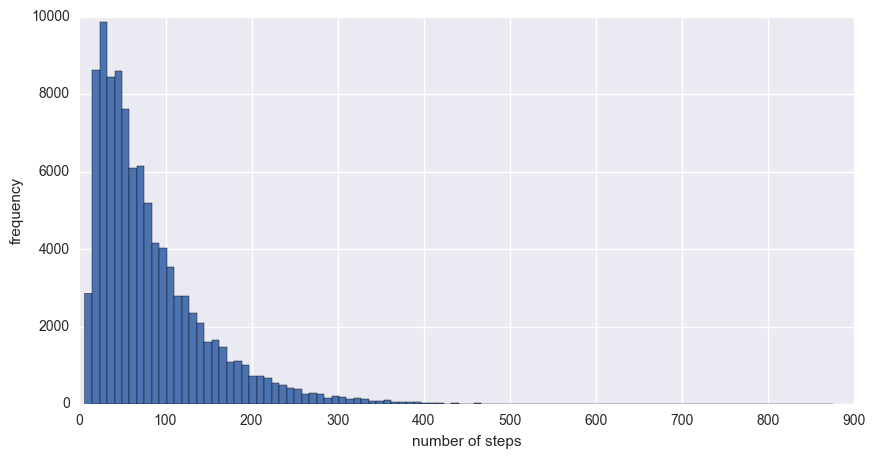
\includegraphics[width=\textwidth]{stopping_time}
        \caption{Stopping time distribution}\label{fig:stop_time}
    \end{figure}

    Fig.~\ref{fig:state_dist} shows the visit distribution over states. The distribution peaks at $500$ since that is the starting state, and tapers off on both sides. This is similar to the plot shown in Fig. 9.1 in~\cite{RLbook}.
    \begin{figure}
        \centering
        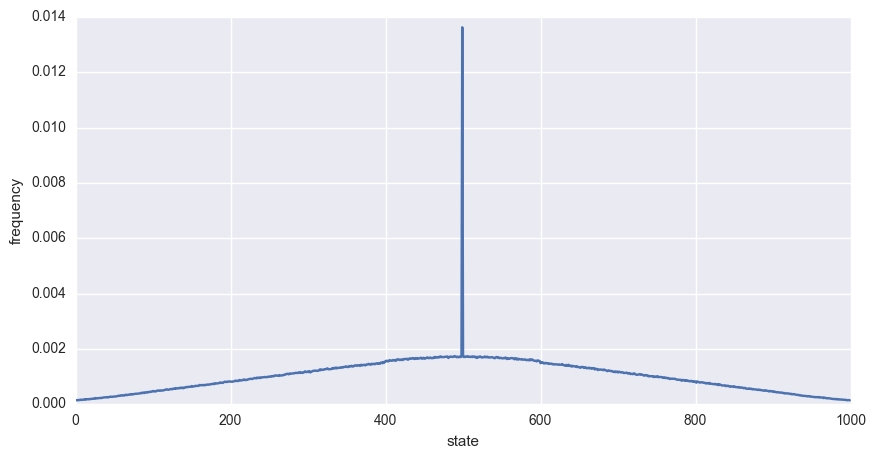
\includegraphics[width=\textwidth]{distribution}
        \caption{State distribution}\label{fig:state_dist}
    \end{figure}

\subsection{Experiment 2}
    In this experiment, we qualitatively inspect how well each of the algorithms do while trying to approximate the value function for the random walk task. We use two different functions.

    The first one is the aggregation function where the states are bucketed. States (1-100) form the first bucket, (101-200) are the second bucket and so on to form a total of 10 buckets. Each bucket has a single value associated with it. State aggregation is a special case of linear function approximation that goes from one hot encoding over the buckets to the estimated value via a linear transform.

    The second function that we use is without any aggregation, i.e.\ we have one value for each state. So this one does not do any function approximation, and can be seen as the best you can do if you had a lot of memory.

    For each of our algorithms, Monte Carlo, semi-gradient $TD(0)$ and demi-gradient $TD(0)$ we show two plots one for each function approximation method. (Fig.~\ref{fig:expt2}). All algorithms are allowed to see 100,000 episodes. For Monte Carlo and semi-gradient $TD(0)$, we use the same alpha values as in~\cite{RLbook}. For the demi-gradient method, best parameters were found by manual tuning. Exact values of parameters can be seen at \url{https://github.com/AshishBora/reinforcement-learning}.

    \begin{figure}
        \centering
        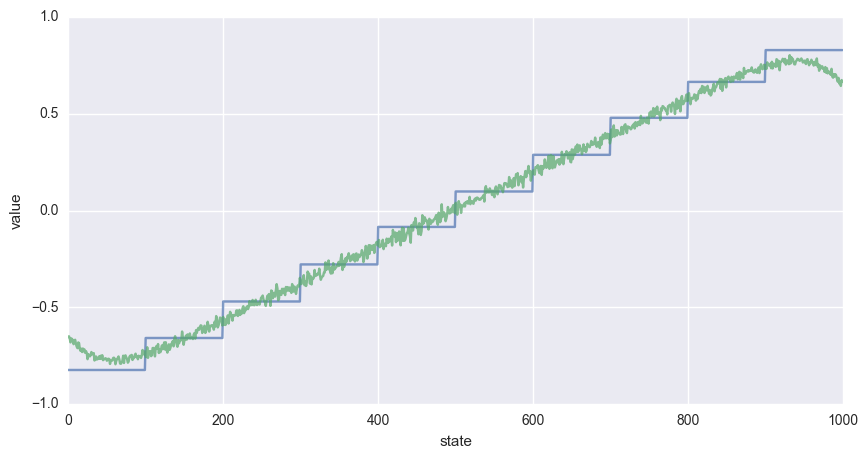
\includegraphics[width=\textwidth]{monte_carlo}
        \caption{Monte Carlo}
        ~
        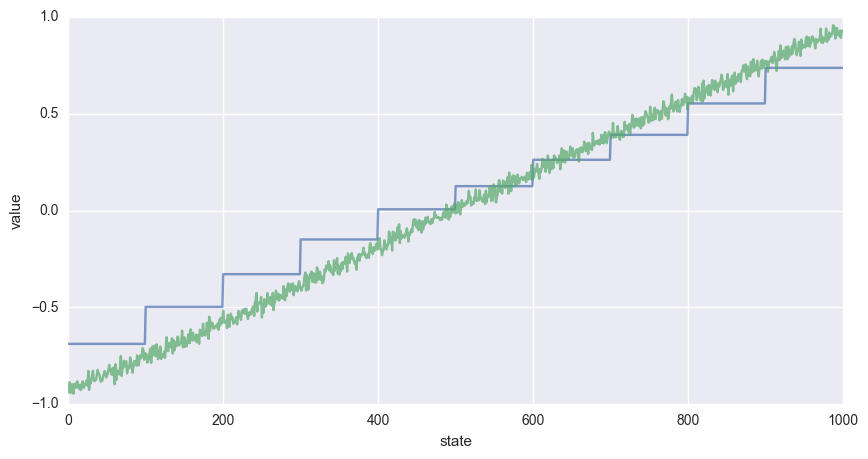
\includegraphics[width=\textwidth]{semi_gradient}
        \caption{semi-gradient $TD(0)$}
        ~
        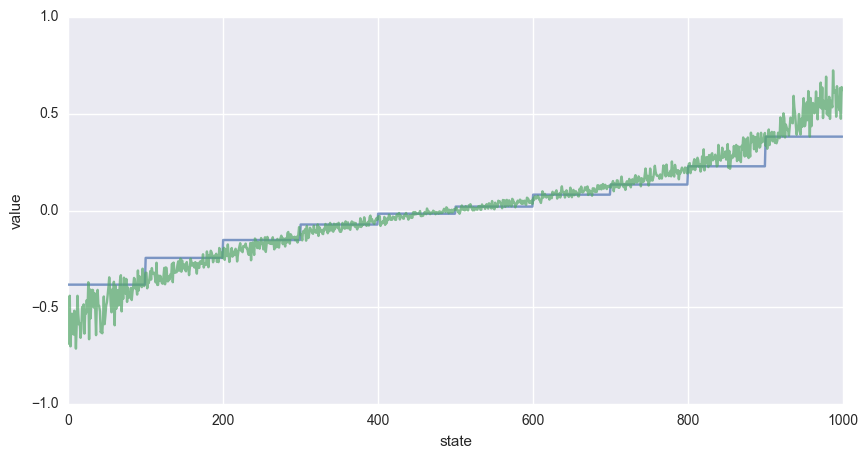
\includegraphics[width=\textwidth]{demi_gradient}
        \caption{demi-gradient $TD(0)$}
        \label{fig:expt2}
    \end{figure}

    For the aggregated function, we observe that Monte Carlo gives the best approximation followed by the semi-gradient and finally demi-gradient is the worst.

    For the second function (no approximation), we see that the semi-gradient is the best followed by Monte Carlo which does slightly worse near the edges and demi-gradient is far from the actual value function.

    It is quite interesting that the convergence is reversed for Monte Carlo and semi-gradient for the two functions. It is also not immediately clear why the demi-gradient method does not do well. We will explore this aspect more in further experiments.

\subsection{Experiment 3}
    In the previous experiment we qualitatively inspected the convergence properties of the three algorithms. In this experiment we seek to quantify those results.

    We use $RMS$ error with respect to the true value function as our metric. Note that this is not the same as the $MSVE$ since we are not weighting by the fraction of time spent in each state.

    To be able to compute the $RMS$, we need to know the true value function. Analytically finding the true value function is easy for the setting where $k=1$ (recall that $k$ was the max hop in one step). In this setting, the optimal value function just linearly increases from $-1$ on the very left to $+1$ on the extreme right. We use $RMS$ using this value function throughout our evaluation.

    Setting $k=1$ leads to very large number of steps when $n = 1000$. Thus, to make the simulation manageable, we chose $n=10$. Plots for $RMS$ error averaged over the states as a function of number of episodes is shown in Fig.\ref{fig:qc1}.
    \begin{figure}
        \centering
        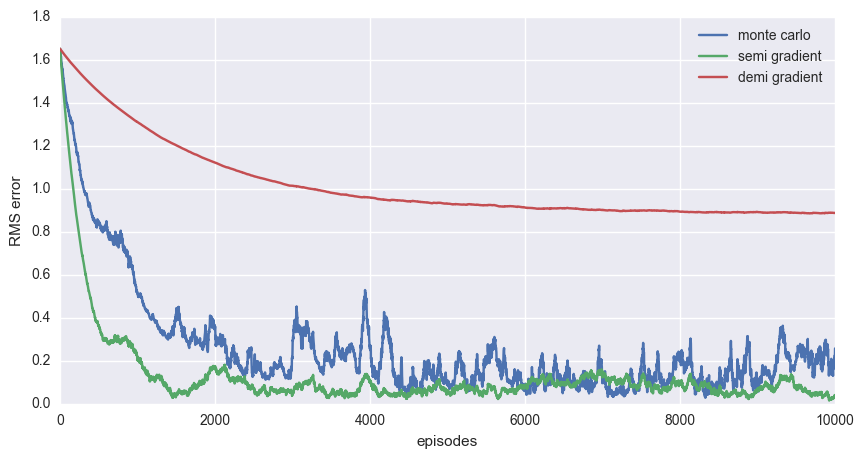
\includegraphics[width=\textwidth]{quant_comp}
        \caption{Quantitative comparison}\label{fig:qc1}
    \end{figure}
    We observe that semi-gradient method does the best on this task, and also has a lower variance. The Monte Carlo method does almost as well, but has a larger variance. Demi-gradient does not do very well and also seems to saturate at a large error. However, it is remarkable that the demi-gradient trajectory is smoother than others, suffering almost no fluctuations at all.


\subsection{Modification to the algorithm}

    In the previous sections, we saw that the demi-gradient algorithm does not do very well. One possible reason for this is that it is doing too much smoothing and hence having a hard time to learn. In fact, we can imagine going continuously from semi-gradient to demi-gradient by introducing one more parameter $\delta$ and writing the update equations as:

    $$\theta \leftarrow \theta + \alpha \left[ R + \gamma \hat{v}(S^{'}, \theta) - \hat{v}(S, \theta) \right] \left[ \nabla \hat{v}(S, \theta) - \gamma \delta \nabla \hat{v}(S^{'}, \theta) \right]$$

    When $\delta = 0$, this is the same as semi-gradient method, and when $\delta=1$, this is the same as demi-gradient method.

    To see how the algorithm behaves as a function of $\delta$, we try several values of $\delta$ on the random walk task and show empirical convergence results. As an additional experiment, we also try negative values of $\delta$.

    The results are shown in Fig.~\ref{fig:qc2}.
    \begin{figure}
        \centering
        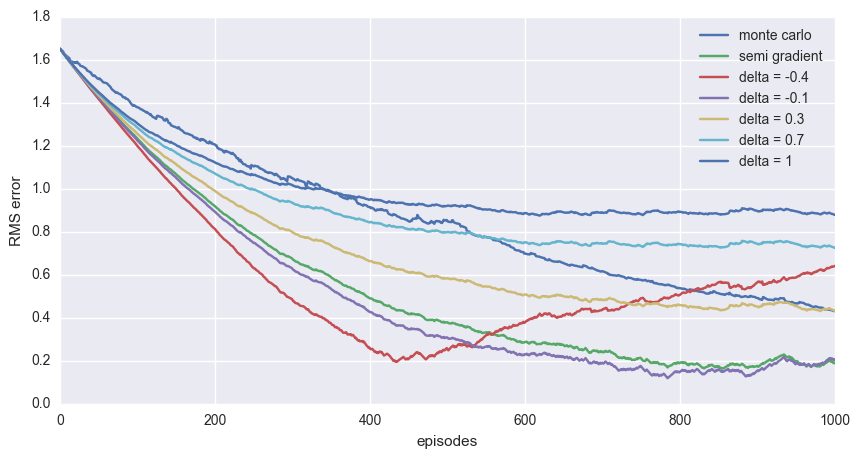
\includegraphics[width=\textwidth]{quant_comp2}
        \caption{Performance for several $\delta$ values}\label{fig:qc2}
    \end{figure}
    We see a very interesting trend here. The performance gets better as $\delta$ decreases i.e.\ as we go from demi-gradient to semi-gradient. But interestingly, the performance further improves when we go to negative values of $\delta$. This trend stops at some point and we start to see that the algorithms with large negative $\delta$ values start to do significantly worse than other algorithms. This suggests an interesting approach to use negative values in the beginning to speed up learning and then increase delta towards $0$ as the algorithm proceeds.


\section{Future Work}
Understanding this idea theoretically can be useful to explain the empirical observations. More experiments on other tasks and settings can validate if negative $\delta$ values are indeed useful, at least as an initialization.


\section{Conclusion}
In this work, we motivated a foundation for the semi-gradient $TD(0)$ algorithm by constructing a new $MSVE$ criterion whose gradient is close to the expectation of the gradient used by the semi-gradient $TD(0)$ algorithm. We then proposed a modification to semi-gradient $TD(0)$ that uses the full gradient of the new criterion. We empirically evaluated this algorithm on a simple random walk task. We also proposed a continuous interpolation between our approach and semi-gradient $TD(0)$ method and empirically studied that spectrum to find a good setting for the interpolation parameter. Surprisingly, we found that going a little bit beyond the spectrum helped get the best performance. Finally, we raise several open questions for future work.
\clearpage

\begin{thebibliography}{9}

\bibitem{RLbook} Richard S. Sutton and Andrew G. Barto, \emph{Reinforcement Learning: An Introduction}, \url{https://webdocs.cs.ualberta.ca/~sutton/book/bookdraft2016sep.pdf}

\end{thebibliography}

\end{document}
